\documentclass[11pt,twoside]{report}


%\newif\ifmynotes
%\mynotesfalse
%\mynotestrue

\usepackage{ece586}


%% TOGGLE  Notes
%\newif\ifgnotes
%\anstrue

%\ifmynotes
%	\definecolor{note_text}{rgb}{1,1,1}		
%	\newcommand{\gskip}{\vspace*{1cm}}
%	\newcommand\gnote[1]{\protect\leavevmode\begingroup\Huge\color{note_text}#1\endgroup\ignorespaces}
%	\newenvironment{gnotes}{\Huge\color{red}}{\ignorespacesafterend}
%\else
%	%\newcommand{\gnote}[1]{#1\ignorespaces} 	% make commands do nothing. 
%	\definecolor{note_text}{rgb}{0,0,.7}
%	\newcommand\gnote[1]{\protect\leavevmode\begingroup\color{note_text}#1\endgroup\ignorespaces}
%	\newenvironment{gnotes}{\color{red}}{\ignorespacesafterend}
%%	\newcommand{\gskip}{}
%\fi
%

\newcommand{\bbN}{{\mathbb{N}}}
\newcommand{\bbR}{{\mathbb{R}}}
\newcommand{\bbQ}{{\mathbb{Q}}}
\newcommand{\bbZ}{{\mathbb{Z}}}
\newcommand{\bbC}{{\mathbb{C}}}
\newcommand{\vecnot}{\underline}
\newcommand{\Id}{{\mathrm{I}}}
\newcommand{\Herm}{{\mathrm{H}}}

\newcommand{\Interior}[1]{\ensuremath{{#1}^{\circ}}}
\newcommand{\Closure}[1]{\ensuremath{\overline{#1}}}
\newcommand{\Complement}[1]{\ensuremath{{#1}^{c}}}

\newcommand{\Real}{\mathrm{Re}}
\newcommand{\Span}{\mathrm{span}}
\newcommand{\Rank}{\mathrm{rank}}
\newcommand{\Nullity}{\mathrm{nullity}}
\newcommand{\Trace}{\mathrm{tr}}
\newcommand{\Diag}{\mathrm{diag}}
\DeclareMathOperator*{\esssup}{ess\,sup}
\DeclareMathOperator*{\minimize}{minimize}

\newcommand{\inner}[2]{{\left\langle #1 \mskip2mu , #2 \right\rangle}}
\newcommand{\tinner}[2]{{\langle #1 \mskip1mu , #2 \rangle}}

\newcommand{\Expect}{\ensuremath{\mathrm{E}}}

\begin{document}

\lectureheader{7}{Representation and Approximation}



\section*{Overview} 

\begin{itemize}
%\item In this lecture, we consider noisy linear observation model
% \[
% \by = A \bx^\star + \be
% \]
% where:
%\begin{itemize}
%\item $\bx^\star$ is an unknown $n$-dimensional vector belonging to a set $\cX \subseteq \reals^n$. 
%\item $A$ is an $m \times n$ measurement matrix
%\item $\be$ is and $m$-dimensional vector of measurement errors
%\end{itemize}


\item This lecture is based on material in  \cite[Chapters 4 and 6]{chamberland:2023EF}%,  \cite[Chapter~7]{luenberger:1997}, and \cite{clarke:2013}
% and \cite[Parts~I--II]{bloch:2011}


\end{itemize}


\section{Best Approximation} 


\begin{itemize}

\item %Let $\vecnot{v}$ be a vector in Banach space $V$ and consider the problem of approximating $
Let $W$ be a a subspace of Banach space $V$. For a vector $\vecnot{v} \in V$ consider the problem of finding an approximation $ \vecnot{w} \in W$ that makes the difference $\vecnot{v} - \vecnot{w}$ as \emph{small} as possible, i.e., 
\[
\minimize \;  \| \vecnot{v} - \vecnot{w} \| \quad \text{subject to  }  \vecnot{w} \in W
\]

\item \textbf{Definition:} A vector $\vecnot{w} \in W$ is called a \textbf{best approximation} of $\vecnot{v}$ if attains the minimum:
\[
\| \vecnot{v} - \vecnot{w} \|  \le \| \vecnot{v} - \vecnot{w}' \|  \quad \text{for all $\vecnot{w}' \in W$}
\]


\item The  following are all possible: 
\begin{itemize}
\item A best approximation does not exists
\item A best approximation exists and is unique (then it is called the best approximation)
\item There are multiple best approximations. 
\end{itemize}
% a best approximation may or may not exist, and if one does exists, it may 

%a best approximation may fail to exist,  it may exist be and unique, or there may be multiple (even countably infinite) best approximations.% And if it does it exit, it may or may not be unique. 

\item \textbf{Example:} Let $X = \bbR^2$ and $W = \{ s (1, 0)  \mid s \in \bbR\}$ be the span of the first standard basis vector. The properties of the best approximation depend on the norm:   
\begin{center}
\begin{tikzpicture}%[>=Stealth]
   \foreach \i in {0,...,2}{
     \begin{scope}[xshift=\i*4.75cm]
      \draw [thick, <->] (-1.2,0)--(2.3,0)node[right] {$W$};;
      \draw [<->] (0,-.5)--(0,2.2);
       \draw [thick, red, ->] (0,0)--(1,1)node[right] {$\vecnot{x}$};
        \draw [very thick, magenta, ->] (0,0)--(1,0) node[below] {$\vecnot{u}$};
%     \draw[red, shorten <=-1cm, shorten >=-3mm] (0,1)--(2,0) node [near end, above] {$\ker A$};
    \end{scope}
   }
   \begin{scope}[draw=blue, thick, densely dashed, xshift = 1cm, yshift = 1cm]
     \draw [] (-1,0)--(0,1)--(1,0)--(0,-1)--cycle;
%     \draw [](4.5,0) circle (0.88cm);
      \draw [](4.75,0) circle (1cm);
     \draw [xshift=9.5cm] (-1,-1) rectangle (1,1);
     
   \end{scope}
   \foreach \i [count=\j from 0] in {1,2,\infty} \scoped [xshift=\j*4.75cm] { \node [anchor=mid west] at (0,-1) {$p=\i$}; };
\end{tikzpicture}
\end{center}

For the point $x = (1,1)$, we have 
\begin{itemize}
\item If $1 \le p  < \infty$ then the  best approximation is unique and given by $\vecnot{w} =  (1 ,0 )$
\item If $p =\infty$  then the best approximation is not unique. Any vector of the from $\vecnot{w} =  (s ,0 )$ for $0 \le s \le 2$ is a best approximation
\end{itemize}


%
%
%\item \textbf{Example:} Let $X = \bbR^2$ and $W = \{ s (1, 1)  \mid s \in \bbR\}$ be the span of the all ones vector. The properties of the best approximation depend on the norm:   
%\begin{center}
%\begin{tikzpicture}%[>=Stealth]
%   \foreach \i in {0,...,2}{
%     \begin{scope}[xshift=\i*4.5cm]
%      \draw [<->] (-1.2,0)--(1.2,0);
%      \draw [<->] (0,-1.2)--(0,1.2);
%%     \draw[red, shorten <=-1cm, shorten >=-3mm] (0,1)--(2,0) node [near end, above] {$\ker A$};
%    \end{scope}
%   }
%   \begin{scope}[draw=blue, thick, densely dashed]
%     \draw [] (-1,0)--(0,1)--(1,0)--(0,-1)--cycle;
%%     \draw [](4.5,0) circle (0.88cm);
%      \draw [](4.5,0) circle (1cm);
%     \draw [xshift=9cm] (-1,-1) rectangle (1,1);
%     
%   \end{scope}
%   \foreach \i [count=\j from 0] in {1,2,\infty} \scoped [xshift=\j*4.5cm] { \node [anchor=mid west] at (0,-1.5) {$p=\i$}; };
%\end{tikzpicture}
%\end{center}
%
%For the point $x = (1,0)$, we have 
%\begin{itemize}
%\item $p =1$ the best approximation is not unique.  Any vector of  the form $\vecnot{w} = (s,s)$ where $0 \le s \le 1$ is a best approximation
%\item $p =2$  best approximation is unique and given by $\vecnot{w} =  (\frac{1}{2} , \frac{1}{2} )$
%\item $p =\infty$  best approximation is unique and given by $\vecnot{w} =  (\frac{1}{2} , \frac{1}{2} )$
%\end{itemize}
%
%

\item \textbf{Example:} %Let $X = \bbR^2$ and $W = \{ \vecnot{x} \mid x_2 = 0\}$ be 
%In the space $\bbR^2$ with with $\ell^1$-norm $\|x\|$
Let $X = \bbR^n$ and  $W  = \{s \vecnot{1} \in \bbR^n \mid  s \in \bbR\}$ be the span of the all ones vector. For a vector  $\vecnot{x}  =(x_1, \dots ,x_n) \in X$ the best approximation  under the $\ell^p$ norm has the form $\vecnot{w}  = s \vecnot{1}$ where the value of $s \in \bbR$  depends on the norm: 
\begin{itemize}
\item  $p =1$  the best approximation is determined by the \emph{median} of the set $\{ x_i \}$. If $n$ is odd then the median is unique but if $n$ is even, then the median can be taken to be any number $s$ that satisfies 
\[
x_{(n/2)} \le s \le x_{(n/2+1)}
\]
where where $x_{(1)} \le x_{(2)} \le \cdots \le x_{(n)}$ the increasing arrangement of $\{ x_i\}$. 
\item Under the $\ell^2$ norm  best approximation is unique and is given by the \emph{arithmetic mean}: 
\[
s = \frac{1}{n} \sum_{i=1}^n x_i 
\]
\item Under the $\ell^\infty$ norm  the best approximation is unique and is given by the midpoint between the minimum and maximum values: 
\[
s =\frac{ \max \{ x_i\} +\min \{ x_i\}}{2} 
\]
\end{itemize}


\item \textbf{Example:} Let $V = \ell^2$ be the Hilbert space of square summable sequences and let $W$ be the span of the standard basis vectors, such that $V$ is equal to the closure of $W$. 
%(Recall that this is the space of all \emph{finite} combinations) %such that $V$ is equal to the closure of $W$. 
For any  $\vecnot{v}  \in V$ that is not in $W$ (i.e., any square summable sequence with an infinite number of nonzero entries) a best approximation of $\vecnot{w}$ in $V$ does not exists. 

%. The sequence $\vecnot{v}  \in V$ defined by $v_i = 1/i^2$, we see that the $\vecnot{v}$ is in the closure of $W$ 

\end{itemize}

\subsection{Orthogonal Projection}

\begin{itemize}


\item  In an arbitrary Banach space, finding a best approximation can be difficult. For the induced norm of a Hilbert space, orthogonal projection simplifies this!


\item Recall that for an inner product space, the \textbf{projection} of $\vecnot{w}$ onto $\vecnot{v}$ is defined by 
\[
\vecnot{u}  =  \displaystyle\frac{\inner{ \vecnot{w} }{ \vecnot{v} }}{\|\vecnot{v}\|^2} \vecnot{v} 
\]
\begin{center}

%$ \vecnot{w} = \displaystyle\frac{\inner{ \vecnot{v} }{ \vecnot{u} }}{\|\vecnot{u}\|^2} \vecnot{u} $ &
\begin{tikzpicture}[scale=0.6]
  \coordinate (v1) at (0,0);
  \coordinate (v2) at (4,3);
  \coordinate (v3) at (6,0);
  \coordinate (v4) at (4,0);
  \coordinate (v5) at (0,3);
  \path[draw] (3.6,0) -- (3.6,0.4) -- (4,0.4);
  \node (v0) at (-0.25,-0.1) {$\vecnot{0}$};
  \draw[-latex,thick] (v1) -- node[at end,above] {$\vecnot{w}$} (v2);
  \draw[-latex,thick] (v1) -- node[at end,below] {$\vecnot{v}$} (v3);
  \draw[-latex,thick] (v1) -- node[at end, below] {$\vecnot{u}$} (v4);
  \draw[thick,dashed] (v4) --  (v2);
  \draw[-latex,thick] (v1) -- node[right,near end] {$\vecnot{w}-\vecnot{u}$} (v5);
\end{tikzpicture}
%\end{tabular}
\end{center}

%\begin{itemize}
%%\item \textbf{Lemma:} 
%\item By construction, the difference between $\vecnot{w}$ and its projection onto $\vecnot{v}$ orthogonal to $\vecnot{v}$, 
%\[
%\inner{ \vecnot{w} - \vecnot{u}}{ \vecnot{v}} = 0  \quad \text{and} \quad \| 
%\]
%
%\item Consequently, if $\vecnot{w}$ is \emph{not} orthogonal to the $\vecnot{v}$, then 
%\[
%\inner{ \vecnot{w}}{ \vecnot{v}}  \ne 0 \quad \implies \quad  \|  \vecnot{w} -  \vecnot{u}\| \le  \|  \vecnot{w} \| 
%\]
%\end{itemize}

%\item \textbf{Lemma:}  
%Let $\vecnot{u}$ be the projection of $\vecnot{w}$ onto $\vecnot{v}$.  
%\[
%\inner{ \vecnot{w}}{ \vecnot{v}}  \ne 0 \quad \implies \quad  \|  \vecnot{w} -  \vecnot{u}\| <   \|  \vecnot{w} \| 
%\]



\item \textbf{Theorem:} Let $V$ be a Hilbert space. For a subset space $W$ and vector $\vecnot{v} \in V$, the following hold: % and $W$ a subspace of $W$. 
%Let $W$ be a subspace of a Hilbert space $V$. For any $\vecnot{v} \in V$ the following hold 

\begin{enumerate}[(1)]

\item  The vector $\vecnot{w} \in W$ is the best approximation of $\vecnot{v} \in V$ by vectors in $W$ if and only if $\vecnot{v} - \vecnot{w}$ is orthogonal to every vector in $W$, i.e., 
\[
\text{$ \vecnot{w}$ is a best approximation} \quad \iff \quad \inner{ \vecnot{v} - \vecnot{w}}{ \vecnot{w'} } = 0 , \quad \text{for all $\vecnot{w}' \in W$}
\] 

\item If a best approximation of $\vecnot{v} \in V$  by vectors in $W$ exists, then it is unique.


\item If $W$ is a closed subspace with a countable orthogonal basis $\vecnot{w}_1, \vecnot{w}_2, \ldots$, then the best approximation of $\vecnot{v}$ by vectors in $W$ exists and is given by
\begin{equation*}
\vecnot{w} = \sum_{i=1}^{\dim (W)} \frac{ \inner{ \vecnot{v} }{ \vecnot{w}_i } }{ \left\| \vecnot{w}_i \right\|^2 } \vecnot{w}_i . 
\end{equation*}
[Note: The implied linear mapping $T \colon V \to W$ defined by $T(\vecnot{v}) = \vecnot{w}$ is called the \textbf{orthogonal projection} of $V$ onto $W$.]
\end{enumerate}


\item \textbf{Proof:} 
\color{blue}
[ See text or hand written notes ]
\color{black} 

\item \textbf{Example:} 
For the standard inner product space $V = \mathbb{R}^3$, let $W$ be the subspace spanned by
\begin{align*}
\vecnot{v}_1 &= (2,2,1), \\
\vecnot{v}_2 &= (3,6,0).
\end{align*}
Then, the Gram-Schmidt process generates the orthogonal basis
\begin{align*}
\vecnot{w}_1 &= (2,2,1), \\
\vecnot{w}_2 &= (-1,2,-2)
\end{align*}
and the orthogonal projection of $\vecnot{v} \in V$ onto $W$ is defined by \vspace{-2mm}
\begin{align*}
T \vecnot{v} &= \sum_{i=1}^2 \frac{ \inner{ \vecnot{v} }{ \vecnot{w}_i } }{ \left\| \vecnot{w}_i \right\|^2 } \vecnot{w}_i \\ &= \frac{1}{9} \inner{ \vecnot{v} }{ (2,2,1) } (2,2,1) + \frac{1}{9} \inner{ \vecnot{v} }{ (-1,2,-2) } (-1,2,-2).
\end{align*}

\newcommand*{\vertbar}{\rule[-1ex]{0.5pt}{2.5ex}}
\item 
Let $V = \bbC^n$ be the standard $n$-dimensional complex Hilbert space and $U \in \bbC^{n\times m}$ be a matrix with orthonormal columns $\vecnot{u}_1,\ldots,\vecnot{u}_m$:

\[ U = \begin{bmatrix} \vertbar & \vertbar & & \vertbar \\ \vecnot{u}_1 & \vecnot{u}_2 & \cdots & \vecnot{u}_m \\ \vertbar & \vertbar & & \vertbar \end{bmatrix} \]

\vspace{4mm}

Then, the best approximation of $\vecnot{v}\in V$ by vectors in $\mathcal{R}(U)$, given by
\begin{equation*}
\vecnot{w} = \sum_{i=1}^m \frac{ \inner{ \vecnot{v} }{ \vecnot{u}_i } }{ \left\| \vecnot{u}_i \right\|^2 } \vecnot{u}_i,
\end{equation*}
can also be written as
\[
 \vecnot{w} = U U^\Herm \vecnot{v} = \sum_{i=1}^m \vecnot{u}_i (\vecnot{u}_i^\Herm \vecnot{v})
  \]


\end{itemize}

\subsection{Projection Operators}


\begin{itemize}
\item \textbf{Definition:} 
A function $F \colon X \rightarrow Y$ with $Y \subseteq X$ is called \textbf{idempotent} if applying the function twice is the same as applying the function once, i.e., 
\[
F(F(x))=F(x)
\]
When $F$ is a linear transformation, this reduces to $F^2 = F \cdot F = F$.

\item \textbf{Definition:} % For a vector space $V$, 
 A \textbf{linear projection} on a vector space $V$ is an idempotent linear operator $T \colon V \rightarrow V$. %is called a \textbf{projection}. 
%Let $V$ be a vector. An  idempotent linear transformation $T \colon V \rightarrow V$ is called  a \textbf{projection}. Since $T = T^2$, it follows that
%\[
%T\vecnot{v} = \vecnot{v} \quad \text{for all $ \vecnot{v} \in \mathcal{R}(T)$}
%\]
% .
%If $T$ is idempotent, then $T$ is called a \textbf{projection} because $T\vecnot{v} = \vecnot{v}$ if $\vecnot{v} \in \mathcal{R}(T)$.

\item \textbf{Note:} In the context of linear algebra, the terms \emph{linear projection} and \emph{projection} are used interchangeably, i.e., projections are assumed to be linear. However, in the broader mathematical context, a projection is any  idempotent (but possibly nonlinear)  operator 


\item \textbf{Example:} For $V = \bbR^3$, the the idempotent matrix $A$ defines a projection onto the first two coordinates. 
\begin{equation*}
A = \begin{bmatrix}
1 & 0 & 1 \\
0 & 1 & 1 \\
0 & 0 & 0
\end{bmatrix}
\end{equation*}


\item \textbf{Theorem:}  
Let $V$ be a vector space and $T \colon V \rightarrow V$ be a  linear projection operator.
Then, the range $\mathcal{R}(T)$ and the  null space $\mathcal{N}(T)$ are disjoint subspaces of $V$.

\item \textbf{Proof:}  
\begin{itemize}
\item Let $\vecnot{v}$ be any vector in the intersection  $ \mathcal{R}(T) \cap  \mathcal{N}(T)$. 
\item Since  $\vecnot{v} \in \mathcal{R}(T)$, there exists $\vecnot{w} \in V$ such that $\vecnot{v} = T\vecnot{w}$. Using the fact that $T$ is a projection, we can write
\[
T\vecnot{v} = T^2  \vecnot{w} = T \vecnot{w} = \vecnot{v}
\]

% means that $T\vecnot{v} = \vecnot{v}$
\item   Meanwhile, the assumption $\vecnot{v}  \in \mathcal{N}(T)$ implies that $T\vecnot{v} = 0$
%\item For any nonzero $\vecnot{v} \in \mathcal{R}(T)$, there is a non-zero $\vecnot{w} \in V$ such that $\vecnot{v} = T\vecnot{w}$. 
%\item  Thus, $T\vecnot{v} = T^2  \vecnot{w} = T \vecnot{w} = \vecnot{v}$ and $T$ projects onto $\mathcal{R}(T)$. Since $\vecnot{v} \neq \vecnot{0}$, we have $\vecnot{v} \notin \mathcal{N}(T)$.
\item Thus, $\vecnot{v}= \vecnot{0}$ and so the two subspaces are disjoint.  
\end{itemize}

\item \textbf{Example:}  
Consider the linear transform $T \colon V \rightarrow V$ defined by $T = \Id - P$, where $P$ is a projection.
It is easy to verify that $T$ is a projection operator because
\[ T^2 = (\Id-P)(\Id-P) = \Id - P- P + P^2 = \Id-P = T \]
In fact, $T$ is a projection onto the null space $\mathcal{N}(P)$ since 
\[
P \vecnot{v} = \vecnot{0} \quad \iff \quad (\Id-P)\vecnot{v} = \vecnot{v}
\]
%$\mathcal{R}(T) = \mathcal{R}(\Id-P) = \mathcal{N}(P)$ because $P \vecnot{v} = \vecnot{0}$ (i.e., $\vecnot{v} \in \mathcal{N}(P)$) if and only if  $(\Id-P)\vecnot{v} = \vecnot{v}$ (i.e., $\vecnot{v} \in \mathcal{R}(T)$).




\item \textbf{Definition:} A linear  projection operator $P \colon V \rightarrow V$ on an inner-product space $V$ is called an \textbf{orthogonal projection} if  the range space $\mathcal{R}(P) $ and  the null space $\mathcal{N}(P)$ are orthogonal subspaces, i.e.,  $\mathcal{R}(P) \perp \mathcal{N}(P)$. 
%Let $V$ be an inner-product space and $P \colon V \rightarrow V$ be a (linear) projection operator. If $\smash{\mathcal{R}(P) \perp \mathcal{N}(P)}$, then $P$ is called an \textbf{orthogonal projection}.


\item \textbf{Example:}
Let $P \colon V \rightarrow V$ be an orthogonal projection.
Since $P\vecnot{v}=\vecnot{0}$ iff $(I-P)\vecnot{v} = \vecnot{v}$, $\mathcal{N}(P) = \mathcal{R}(I-P)$.
Thus, $P \vecnot{v} \in \mathcal{R}(P)$ is orthogonal to $(I-P) \vecnot{v} \in \mathcal{N}(P)$.




\item \textbf{Theorem:} 
For $V=F^n$ with the standard inner product, a projection matrix $P$ is an orthogonal projection matrix if and only if it is Hermitian, i.e. $P^\Herm = P$.



\item \textbf{Proof:} 
\begin{itemize}
\item If $P=P^\Herm$, then $P = P^2 = P^\Herm P$ and $\mathcal{R}(P) \perp \mathcal{N}(P)$ follows from
\[ \tinner{ P\vecnot{u} }{ (I-P)\vecnot{v} } = \vecnot{v}^\Herm (I-P)^\Herm P \vecnot{u} = \vecnot{v}^\Herm (P - P^\Herm P) \vecnot{u} = 0.  \]
\item  If $\mathcal{R}(P) \perp \mathcal{N}(P)$, then $P=P^\Herm$ because  $\tinner{P\vecnot{u}}{\vecnot{v}} = \tinner{\vecnot{u}}{P\vecnot{v}}$ for all $\vecnot{u},\vecnot{v}$ by 
\[ \tinner{P\vecnot{u}}{\vecnot{v}} = \tinner{P\vecnot{u}}{P\vecnot{v}+(I-P)\vecnot{v}} = \tinner{P\vecnot{u}}{P\vecnot{v}} + \tinner{P\vecnot{u}}{(I-P)\vecnot{v}} = \tinner{P \vecnot{u}}{P \vecnot{v}}. \qedhere \]
\end{itemize}



\end{itemize}


\section{Least-Squares Solutions of Linear System}

\begin{itemize}

\item For approximation by  a  finite-dimensional  subspace, the the best approximation problem has a natural matrix representation. 



\item  \textbf{Theorem:} Let $V$ be a Hilbert space and $\vecnot{w}_1 ,\vecnot{w}_2 , \ldots, \vecnot{w}_n$ be a basis for subspace $W$.
For any $\vecnot{v} \in V$, the best approximation of $\vecnot{v}$ in $W$ is given by
\[
\hat{v} = \sum_{i=1}^n s_i \vecnot{w}_i
\]
where $s_1, \dots, s_n$ can be found by solving the following system of linear equations: 
\begin{equation} \label{eq:least_squares}
%\label{eqn:DualNormalEquations}
\left[ \begin{array}{cccc}
\inner{ \vecnot{w}_1 }{ \vecnot{w}_1 }
& \inner{ \vecnot{w}_2 }{ \vecnot{w}_1 } & \cdots
& \inner{ \vecnot{w}_n }{ \vecnot{w}_1 } \\
\inner{ \vecnot{w}_1 }{ \vecnot{w}_2 }
& \inner{ \vecnot{w}_2 }{ \vecnot{w}_2 } & \cdots
& \inner{ \vecnot{w}_n }{ \vecnot{w}_2 } \\
\vdots & \vdots & \ddots & \vdots \\
\inner{ \vecnot{w}_1 }{ \vecnot{w}_n }
& \inner{ \vecnot{w}_2 }{ \vecnot{w}_n } & \cdots
& \inner{ \vecnot{w}_n }{ \vecnot{w}_n }
\end{array} \right]
\left[ \begin{array}{c}
s_1 \\ s_2 \\ \vdots \\ s_n \end{array} \right]
= \left[ \begin{array}{c}
\inner{ \vecnot{v} }{ \vecnot{w}_1 } \\
\inner{ \vecnot{v} }{ \vecnot{w}_2 } \\ \vdots \\
\inner{ \vecnot{v} }{ \vecnot{w}_n } \end{array} \right] .
\end{equation}

\item \textbf{Proof:} 

\begin{itemize}
\item The projection theorem shows that $\hat{\vecnot{v}} \in W$ is the best approximation of $\vecnot{v} \in V$ if and only if the error is orthogonal to the $W$, i.e., 
\[
(\vecnot{v} - \hat{\vecnot{v}}) \perp \vecnot{w}_j \quad \text{ for $j=1,\ldots,n$}
\]
\item Equivalently
\begin{equation*}
\inner{ \vecnot{v} - \hat{\vecnot{v}} }{ \vecnot{w}_j }
= \inner{ \vecnot{v} - \sum_{i=1}^n s_i \vecnot{w}_i }{ \vecnot{w}_j }
= 0 \vspace{-1mm}
\end{equation*}
\item Rearranging and using linearity of the inner product in its first argument leads to the so-called  \textbf{normal equations}:
\begin{equation*}
\sum_{i=1}^n s_i \inner{ \vecnot{w}_i }{ \vecnot{w}_j }
= \inner{ \vecnot{v} }{ \vecnot{w}_j }, \quad \text{for $ j=1,\ldots,n$}
\end{equation*}

%\item 
%This gives a system of $n$ linear equations in $n$ unknowns $s_1, \dots, s_n$ defined by
%\begin{equation*}
%\underbrace{\left[ \begin{array}{cccc}
%\inner{ \vecnot{w}_1 }{ \vecnot{w}_1 }
%& \inner{ \vecnot{w}_2 }{ \vecnot{w}_1 } & \cdots
%& \inner{ \vecnot{w}_n }{ \vecnot{w}_1 } \\
%\inner{ \vecnot{w}_1 }{ \vecnot{w}_2 }
%& \inner{ \vecnot{w}_2 }{ \vecnot{w}_2 } & \cdots
%& \inner{ \vecnot{w}_n }{ \vecnot{w}_2 } \\
%\vdots & \vdots & \ddots & \vdots \\
%\inner{ \vecnot{w}_1 }{ \vecnot{w}_n }
%& \inner{ \vecnot{w}_2 }{ \vecnot{w}_n } & \cdots
%& \inner{ \vecnot{w}_n }{ \vecnot{w}_n }
%\end{array} \right]}_G
%\underbrace{\left[ \begin{array}{c}
%s_1 \\ s_2 \\ \vdots \\ s_n \end{array} \right]}_{\vecnot{s}}
%= \underbrace{\left[ \begin{array}{c}
%\inner{ \vecnot{v} }{ \vecnot{w}_1 } \\
%\inner{ \vecnot{v} }{ \vecnot{w}_2 } \\ \vdots \\
%\inner{ \vecnot{v} }{ \vecnot{w}_n } \end{array} \right]}_{\vecnot{t}} .
%\end{equation*}
\end{itemize}


\item \textbf{Remark:} Recall that a Hilbert space is a complete inner product space.
\begin{itemize}
\item The fact that $\vecnot{w}_1, \dots, \vecnot{w}_n$ is a basis for $W$ does not depend on the  inner product, since linear independence and span are basic properties of the underlying vector space.% (i.e., they do not depend on the inner product).

\item  However, if one replaces the original inner product with a new one (e.g., by reweighing) then this changes the induced norm as well as the best approximation. 

\end{itemize}

\item The system of linear equations in \eqref{eq:least_squares}  can be written compactly as
\[
G \vecnot{s} = \vecnot{t} 
\]
where $t_i = \inner{ \vecnot{v} }{ \vecnot{w}_j }$ for $j = 1, \dots, n$ and  the $n \times n$ matrix $G$ is called the \textbf{Gramian matrix}:
% For $\vecnot{w}_1,\ldots,\vecnot{w}_n$, the $n \times n$ \textbf{Gramian matrix} is defined to be
\begin{equation*}
G = \left[ \begin{array}{cccc}
\inner{ \vecnot{w}_1 }{ \vecnot{w}_1 }
& \inner{ \vecnot{w}_2 }{ \vecnot{w}_1 } & \cdots
& \inner{ \vecnot{w}_n }{ \vecnot{w}_1 } \\
\inner{ \vecnot{w}_1 }{ \vecnot{w}_2 }
& \inner{ \vecnot{w}_2 }{ \vecnot{w}_2 } & \cdots
& \inner{ \vecnot{w}_n }{ \vecnot{w}_2 } \\
\vdots & \vdots & \ddots & \vdots \\
\inner{ \vecnot{w}_1 }{ \vecnot{w}_n }
& \inner{ \vecnot{w}_2 }{ \vecnot{w}_n } & \cdots
& \inner{ \vecnot{w}_n }{ \vecnot{w}_n }
\end{array} \right] \vspace{-1mm}
\end{equation*}
%This matrix 
%Since $g_{ij} =\inner{ \vecnot{w}_j }{ \vecnot{w}_i }$, we see $G$ is Hermitian symmetric (i.e. $G^\Herm = G$).


%\end{itemize}




%\item  Let $W$ be a subspace of a Hilbert space $V$ that is spanned by the linearly independent (but not necessarily  orthogonal) set of vectors  $\vecnot{w}_1, \ldots, \vecnot{w}_n \in V$.



%\item \textbf{Definition:}  For $\vecnot{w}_1,\ldots,\vecnot{w}_n$, the $n \times n$ \textbf{Gramian matrix} is defined to be
%\begin{equation*}
%G = \left[ \begin{array}{cccc}
%\inner{ \vecnot{w}_1 }{ \vecnot{w}_1 }
%& \inner{ \vecnot{w}_2 }{ \vecnot{w}_1 } & \cdots
%& \inner{ \vecnot{w}_n }{ \vecnot{w}_1 } \\
%\inner{ \vecnot{w}_1 }{ \vecnot{w}_2 }
%& \inner{ \vecnot{w}_2 }{ \vecnot{w}_2 } & \cdots
%& \inner{ \vecnot{w}_n }{ \vecnot{w}_2 } \\
%\vdots & \vdots & \ddots & \vdots \\
%\inner{ \vecnot{w}_1 }{ \vecnot{w}_n }
%& \inner{ \vecnot{w}_2 }{ \vecnot{w}_n } & \cdots
%& \inner{ \vecnot{w}_n }{ \vecnot{w}_n }
%\end{array} \right] \vspace{-1mm}
%\end{equation*}
%Since $g_{ij} =\inner{ \vecnot{w}_j }{ \vecnot{w}_i }$, we see $G$ is Hermitian symmetric (i.e. $G^\Herm = G$).
%
%


\item \textbf{Definition:}  A matrix $M\in F^{n \times n}$ is \textbf{positive-semidefinite} if $M=M^\Herm$ and $\vecnot{v}^\Herm M \vecnot{v} \geq 0$ for all $\vecnot{v} \in F^n - \left\{ \vecnot{0} \right\}$.
If the inequality is strict, then it is \textbf{positive-definite}.


\item \textbf{Theorem:}
A Gramian matrix $G$ is always positive-semidefinite. Furthermore, it is positive-definite if and only if the vectors $\vecnot{w}_1, \ldots, \vecnot{w}_n$ are linearly independent.

\item \textbf{Proof:} 
For any $\vecnot{v}\in V$, 
\begin{align*}
\vecnot{v}^\Herm G \vecnot{v} & = \sum_i \sum_j \overline{ v}_i g_{ij} v_j \\
& = \sum_i \sum_j \overline{ v}_i  \inner{ \vecnot{w}_j}{ \vecnot{w}_i   }  v_j \\
&=  \inner{ \sum_j v_j \vecnot{w}_j  }{  \sum_i  v_i \vecnot{w}_i    } \\
& = \Big \| \sum_j v_j \vecnot{w}_j \Big\|^2
\end{align*}
Recall that vectors $\vecnot{w}_1, \ldots, \vecnot{w}_n$ are linearly independent if an only if $\sum_j v_j \vecnot{w}_j =  \vecnot{0}  \iff \vecnot{v} = \vecnot{0}$
 
 
\item \textbf{Example:} Consider the Hilbert space $V = F^n$ with standard inner product and let  $A \in F^{m \times n}$ be a matrix whose $i$-th column is $\vecnot{w}_i \in V$.

\begin{itemize}
\item 
A vector  $\hat{\vecnot{v}} \in W = \text{colspace}(A)$ can be written as 
\[ \hat{\vecnot{v}} = A \vecnot{s} = \sum_{i=1}^n s_i \vecnot{w}_i.
\]

\item The best approximation of $\vecnot{v}$ by vectors in $W$ is found by solving
\[ \min_{\hat{\vecnot{v}}\in W} \| \vecnot{v} - \hat{ \vecnot{v}} \| = \min_{\vecnot{s} \in F^n} \| \vecnot{v} - A \vecnot{s} \|  \]

\item 
For the induced norm, any solution must satisfy the normal equations
\[ \inner{ \vecnot{v} - \hat{\vecnot{v}} }{ \vecnot{w}_j }
= \inner{ \vecnot{v} - A \vecnot{s} }{ \vecnot{w}_j }
= 0, \quad j \in [n]
\]



\item These equations can be expressed as
\begin{equation*}
\vecnot{0} = \left[ \begin{array}{c} \vecnot{w}_1^\Herm \\ \vdots \\ \vecnot{w}_n^\Herm \end{array} \right] \left( \vecnot{v} - A \vecnot{s} \right) = A^\Herm \vecnot{v} - A^\Herm A \vecnot{s} = \vecnot{t} - G \vecnot{s},
\end{equation*}
where$G = A^\Herm A$ and  $\vecnot{t} \coloneqq  A^\Herm \vecnot{v}$ %is sometimes called the the \textbf{cross-correlation vector.}


\item If the columns  $\vecnot{w}_1, \ldots, \vecnot{w}_n$ are linearly independent, the Gramian matrix is positive definite and hence invertible.
Thus, the solution to the system of linear equations is given by % optimal solution for the least-squares problem is given by
\begin{equation*}
\vecnot{s} = G^{-1} \vecnot{t} = \left( A^\Herm A \right)^{-1} A^\Herm \vecnot{v},
\end{equation*}
%Here,  the matrix $\left( A^\Herm A \right)^{-1} A^\Herm$ is pseudoinverse} of $A$ in this case.

\item Finally, the best approximation of $\vecnot{v} \in V$ by vectors in $W$ is 
\begin{equation*}
\hat{\vecnot{v}} = A \vecnot{s} = A \left( A^\Herm A \right)^{-1} A^\Herm \vecnot{v} 
\end{equation*}
\item Here, we see that the matrix \textbf{$P = A \left( A^\Herm A \right)^{-1} A^\Herm$ is the projection matrix} for the range of $A$. It defines an orthogonal projection onto the range of $A$ (i.e., the subspace spanned by the columns of $A$).


\end{itemize} 
\end{itemize}

\subsection{Weighted Least-Squares} 

\begin{itemize}

\item 
For the standard Euclidean norm $\| \vecnot{v} \|_E = \sqrt{\vecnot{v}^\Herm \vecnot{v}}$ and any invertible $B$, consider the weighted least-squares problem
\[ \min_{\hat{\vecnot{v}}\in W} \| B(\vecnot{v} - \hat{ \vecnot{v}}) \|_E = \min_{\vecnot{s}} \| B( \vecnot{v} - A \vecnot{s}) \|_E \]
But, $\| B \vecnot{v} \|_E$ equals the induced norm $\| \vecnot{v} \|$ for the weighted inner product
\[ \inner{ \vecnot{u} }{ \vecnot{v} }  \coloneqq \vecnot{v}^\Herm B^\Herm B \vecnot{u}. \]

\item 
For the weighted inner product, the normal equations look the same
\[ \inner{ \vecnot{v} - \hat{\vecnot{v}} }{ \vecnot{w}_j }
= \inner{ \vecnot{v} - A \vecnot{s} }{ \vecnot{w}_j }
= 0, \quad j \in [n]. \]
but they solve a different problem and they reduce to
\begin{equation*}
\vecnot{0} = \left[ \begin{array}{c} \vecnot{w}_1^\Herm \\ \vdots \\ \vecnot{w}_n^\Herm \end{array} \right] B^\Herm B \left( \vecnot{v} - A \vecnot{s} \right) = A^\Herm B^\Herm B \vecnot{v} - A^\Herm B^\Herm B A \vecnot{s}
\end{equation*}
\end{itemize}

\subsection{Linear Minimum Mean-Squared Error} 

\begin{itemize}
\item  Let $Y, X_1, \ldots, X_n$ be zero-mean random variables.
Linear minimum mean-squared error (LMMSE) estimation finds $s_1, \ldots, s_n$ such that
\[ \hat{Y} = s_1 X_1 + \cdots + s_n X_n \]
minimizes the mean squared-error $\Expect[|Y-\hat{Y}|^2]$.
\item Using the inner product
\begin{equation*}
\inner{ X }{ Y } = \Expect \left[ X \overline{Y} \right],
\end{equation*}
the normal equations for the LMMSE estimate $\hat{Y}$ are $G \vecnot{s} = \vecnot{t}$, where
\begin{equation*}
G = \left[ \begin{array}{cccc}
\Expect \left[ X_1 \overline{X}_1 \right]
& \Expect \left[ X_2 \overline{X}_1 \right] & \cdots
& \Expect \left[ X_n \overline{X}_1 \right] \\
\Expect \left[ X_1 \overline{X}_2 \right]
& \Expect \left[ X_2 \overline{X}_2 \right] & \cdots
& \Expect \left[ X_n \overline{X}_2 \right] \\
\vdots & \vdots & \ddots & \vdots \\
\Expect \left[ X_1 \overline{X}_n \right]
& \Expect \left[ X_2 \overline{X}_n \right] & \cdots
& \Expect \left[ X_n \overline{X}_n \right] \\
\end{array} \right], \quad \vecnot{t} = \left[ \begin{array}{c}
\Expect \left[ Y \overline{X}_1 \right] \\
\Expect \left[ Y \overline{X}_2 \right] \\ \vdots \\
\Expect \left[ Y \overline{X}_n \right] \end{array} \right].
\end{equation*}

\item If $G$ is invertible, then $\vecnot{s} = G^{-1} \vecnot{t}$ implies $\Expect [|\hat{Y}|^2] = \vecnot{s}^\Herm G \vecnot{s} = \vecnot{s}^\Herm \vecnot{t}$ and
\begin{equation*}
%\left\| Y - \hat{Y} \right\|^2 =
\left\| Y \right\|^2 -\| \hat{Y} \|^2 
= \Expect[ |Y|^2 ]
- \Expect[ |\hat{Y}|^2 ] = \Expect \left[ |Y|^2 \right] - \vecnot{s}^\Herm \vecnot{t}.
\end{equation*}

\end{itemize}

\subsection{Dual Approximations} 

\begin{itemize}

\item An underdetermined system of linear equations has an infinite number of solutions.
It often makes sense to prefer the \textbf{minimum-norm solution}.



\item Let $V$ be a Hilbert space and $\vecnot{w}_1 ,\vecnot{w}_2 , \ldots, \vecnot{w}_n$ be a basis for $W\subseteq V$.
For a vector $\vecnot{c} \in F^n$, the \textbf{dual approximation} problem is given by %to find the minimum-norm vector $\vecnot{w}\in V$ satisfying $\inner{ \vecnot{w} }{ \vecnot{w}_i } = c_i$ for $i=1,\ldots,n$, i.e., 
\[
\minimize_{\vecnot{w} \in  V  } \quad \| \vecnot{w} \| \quad \text{subject to} \quad \inner{ \vecnot{w} }{ \vecnot{w}_i } = c_i \quad \text{for $i = 1, \dots , n$}
\]

\item \textbf{Theorem:} 
%Let $V$ be a Hilbert space and $\vecnot{w}_1 ,\vecnot{w}_2 , \ldots, \vecnot{w}_n$ be a basis for $W\subseteq V$.
%The \textbf{dual approximation} problem is to find the minimum-norm vector $\vecnot{w}\in V$ satisfying $\inner{ \vecnot{w} }{ \vecnot{w}_i } = c_i$ for $i=1,\ldots,n$.
The solution $\vecnot{w}$ to the dual approximation problem  satisfies 
\[ \vecnot{w} = \sum_{i=1}^n s_i \vecnot{w}_i %\in W,
  \]
where $s_1,s_2,\ldots,s_n$ can be found by solving \eqref{eq:least_squares} with $\inner{ \vecnot{v} }{ \vecnot{w}_i } = c_i$.

\item \textbf{Example: } For $A \in \mathbb{C}^{m\times n}$ with $m<n$ and $\vecnot{v} \in \mathbb{C}^m$, consider the underdetermined linear system $A \vecnot{s} = \vecnot{v}$.
Then, the dual approximation theorem can be applied to solve the minimum-norm problem
\[% \min_{\vecnot{s}\,  : \, A\vecnot{s} = \vecnot{v}} \| \vecnot{s} \|
\minimize_{\vecnot{s} \in  \bbC^n  } \quad  \| \vecnot{s}\| \quad \text{subject to} \quad A\vecnot{s} = \vecnot{v}
 \]


\begin{itemize} 
\item  To see this as a dual approximation, we can rewrite the constraint $A \vecnot{s} = \vecnot{v}$ as $B^\Herm \vecnot{s} = \vecnot{v}$ where $B = A^\Herm$.
Then, the theorem concludes that the minimum-norm solution lies in  the column space of $B=A^\Herm$.



\item 
Using $\vecnot{s} \in \mathcal{R}(A^\Herm)$, there is a $\vecnot{t}$ such that $\hat{\vecnot{s}} = A^\Herm \vecnot{t}$ and the constraint gives $A (A^\Herm \vecnot{t}) = \vecnot{v}$.
If the rows of $A$ are linearly independent, then the columns of $B=A^\Herm$ are linearly independent and $(B^\Herm B)^{-1} = (A A^\Herm)^{-1}$ exists.



\item Thus, the solution $\hat{\vecnot{s}}$ can be obtained in closed form and is given by \vspace{-1mm}
\[
 \hat{\vecnot{s}} = A^\Herm \left( A A^\Herm \right)^{-1} \vecnot{v}
 \]

\end{itemize}


\end{itemize}



\section{Four Fundamental Subspaces} 


\begin{itemize}

\item A matrix $A \in \bbR^{m \times n}$ defines \textbf{four fundamental subspaces} 
\begin{itemize}
\item The column space (a.k.a.\ range) 
\[
\cR(A)  \coloneqq \{ A \vecnot{x} \mid \vecnot{x} \in \bbR^n  \} 
\]
\item The row space (a.k.a.\ range transpose) 
\[
\cR(A^\top )  \coloneqq \{ A^\top  \vecnot{y} \mid \vecnot{y} \in \bbR^m  \} 
\]
\item The null space 
\[
\cN(A)  \coloneqq \{ \vecnot{x} \in \bbR^n \mid A \vecnot{x} = \vecnot{0} \} 
\]
\item The null space of the transpose
\[
\cN(A^\top)  \coloneqq \{ \vecnot{y} \in \bbR^m \mid A^\top \vecnot{y} = \vecnot{0} \} 
\]
\end{itemize}


\item \textbf{Lemma:} For a matrix $A$, 
\begin{enumerate}[(i)]
\item The null space $\cN(A)$ is the orthogonal complement of the row space $\cR(A^\top)$, i.e., these subspaces are orthogonal to each other and  every $\vecnot{x} \in \bbR^n$ has unique decomposition 
\[
\vecnot{x} =  \vecnot{x}_r + \vecnot{x}_n \quad  \vecnot{x}_r \in \cR(A^\top)\quad  \vecnot{x}_n \in \cN(A)
\]
\item The null space of the transpose $\cN(A^\top )$ is the orthogonal complement of the column space $\cR(A)$%, i.e., these subspaces are orthogonal to each other and  every $\vecnot{x} \in \bbR^n$ has unique decomposition 
%\[
%\vecnot{x} =  \vecnot{x}_r + \vecnot{x}_n \quad  \vecnot{x}_r \in \cR(A^\top)\quad  \vecnot{x}_n \in \cN(A)
%\]
\end{enumerate}

\item \textbf{Proof:}
\begin{itemize}
\item If $\vecnot{x} \in \mathbb{R}^n$ is in the null space of $A$  then all the rows of $A$ orthogonal to $\vecnot{x}$, i.e., 
\[ A \vecnot{x} = \begin{bmatrix} -- \text{row  $1$} -- \\ -- \text{row $2$} -- \\ \vdots \\ -- \text{row $m$} -- \end{bmatrix} \begin{bmatrix}x_1 \\ x_2 \\ \vdots \\ x_n \end{bmatrix} = \begin{bmatrix} 0 \\ 0 \\ \vdots \\ 0 \end{bmatrix} \]
%and this implies that  $\cN(A)  \subseteq \mathcal{R}(A^\top)^\perp$

%\item Alternatively, if $\vecnot{x} \in  \mathcal{R}(A^\top)^\perp$ then $\inner{\vecnot{x}}{ \vecnot{w} } = 0$ for all $\vecnot{w} \in \cR(A^\top)$. 

\item  Part (ii) follows from applying  part (i) to $A^\top$
\end{itemize}


\item Recall that the rank of an $m \times n$  matrix $A$ is 
\begin{align*}
\rank (A) = \dim( \cR(A)) = \dim(\cR(A^\top))
\end{align*}
Hence, the above lemma recovers the rank-nullity theorem:
\begin{align*}
\dim(\cN(A))   & = n - \rank(A) \\
\dim(\cN(A^\top)) & = m - \rank(A) 
%\rank (A) +   =
\end{align*}

\begin{center}
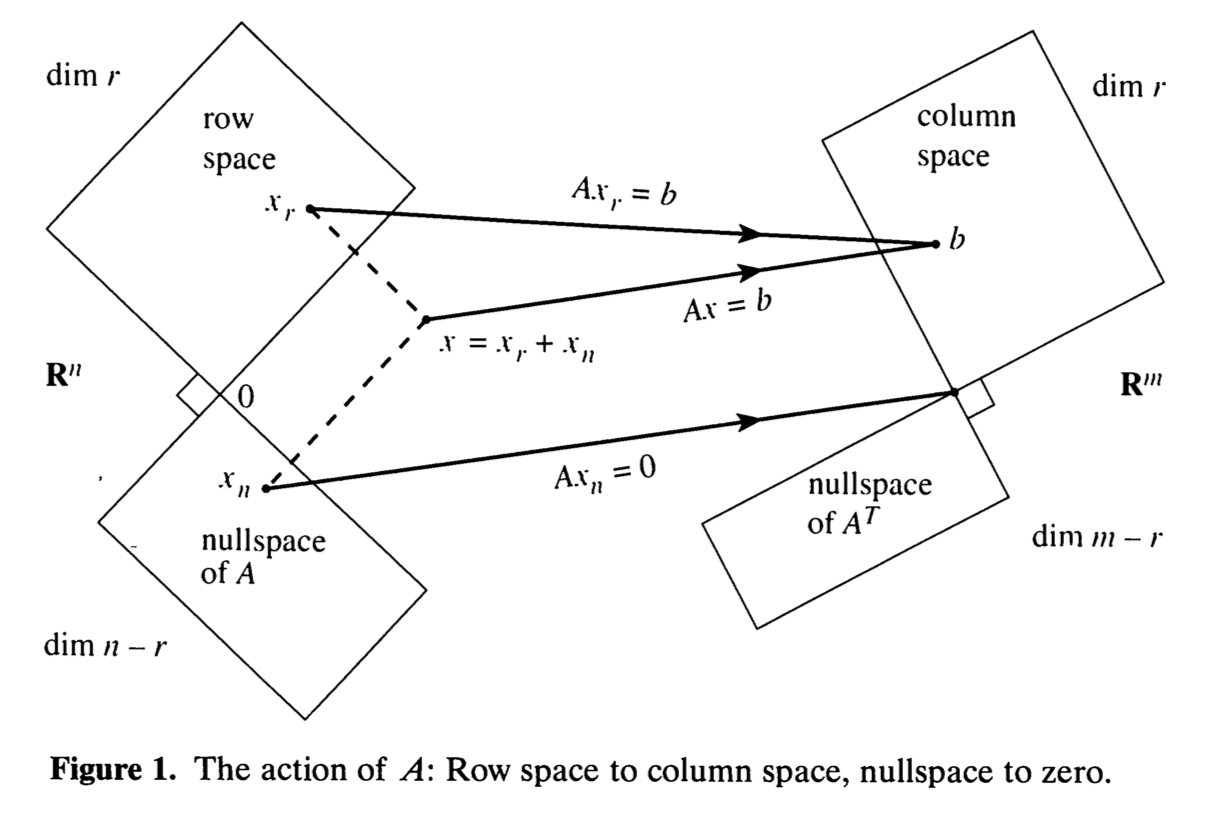
\includegraphics[width = 5in]{figures/strang_fig1.png}
\end{center}
[{\footnotesize Figure from ``The Fundamental Theorem of Linear Algebra'' by Gilbert Strang, The American Mathematical Monthly, Nov. 1993} ]

%
%
\includegraphics[width=105mm]{figures/strang_fig2}



\item  \textbf{Definition:} Let  $(V, \inner{\cdot}{\cdot}_V)$ and $(W, \inner{\cdot}{\cdot}_w)$ be Hilbert spaces, and assume $T \colon V \rightarrow W$ is a continuous linear transformation (i.e., $\| T \|_{\mathrm{op}} < \infty$).
Then, the \textbf{adjoint} $T^*$ is the unique linear transformation mapping $W$ to $V$ such that \vspace{-2mm}
\begin{equation*}
\inner{ T \vecnot{v} }{ \vecnot{w} }_W
= \inner{ \vecnot{v} }{ T^* \vecnot{w} }_V \quad\quad \text{for all }\vecnot{v} \in V, \vecnot{w} \in W
\end{equation*}



\item \textbf{Fact:} For every $\vecnot{v} \in V$, the following 3 conditions are equivalent:
\begin{enumerate}[(i)]
\item $\vecnot{v} \in \mathcal{N}(T)$
\item $\inner{ \vecnot{v} }{ T^* \vecnot{w} }_V = 0$ for all  $\vecnot{w} \in W$
\item $\vecnot{v} \in \mathcal{R}(T^*)^\perp$


% because $\inner{ \vecnot{v} }{ T^* \vecnot{w} }_V = \inner{ T \vecnot{v} }{ \vecnot{w} }_W = 0$ for all $\vecnot{w} \in W$
\end{enumerate}
\end{itemize}



\bibliographystyle{alpha}%{IEEEtran}
\bibliography{/Users/galenreeves/Dropbox/Library/long_names,/Users/galenreeves/Dropbox/Library/library} 
\end{document}

